\chapter{Related Works}

\section{Data Mining}

Data mining \cite{zaki2010advances}\cite{han2011data} is an interdisciplinary subfield of computer science and statistics, that is represented as a process of discovering patterns and inferences in large data sets. It is designed to extract information from a data set and transform it into a comprehensible structure for further use. \medskip

Data mining is a tool for information extraction, processing, representation and summarization. 

\medskip \noindent Stages of data mining:
\begin{verse}
	$\bullet$ Selection: The information that seems to be useful for the prediction needs to be selected.\\
	$\bullet$ Preprocessing: The dataset may include errors, missing values or inconsistent data that need to be filtered out.\\
	$\bullet$ Transformation: Some features of the dataset need some transformation, like normalization, to get an appropriate form.\\
	$\bullet$ Data mining: Now the data mining techniques need to be used that can discover the patterns.\\
	$\bullet$ Evaluation: The patterns are known hence it can be seen not all of them are needed for the prediction.
\end{verse}

Data mining has applications in multiple fields, not just like in science and research, but also in business, banking, manufactoring, insurance and so on. It can help companies to develop more effective strategies in a more optimal way.



\subsection{The Dataset}

Selecting the appropriate information that can be useful for the dataset is not as easy as it seems. A well-defined dataset is large-scale and carries a lot of information whereof patterns can be predicted. Collecting enough relevant data is a long process, but there are public datasets that can be used for free. \medskip

Online News Popularity dataset \cite{Fernandes2015API} - which is a prediction of Mashable news popularity - is publicly available at UCI Machine Learning repository. It aims on predicting the future popularity of news articles from given information that are known before the release of news articles. \smallskip

Mashable is a digital media website that is founded in 2005. Online News Popularity dataset \cite{Ren2015PredictingAE} contains information about 40.000 articles published between 2013 and 2015 on Mashable's website. \smallskip

Online News Popularity dataset consists of 58 predictive features, 2 other attributes of accessory information and 1 goal field, which is the number of shares. There were nominal features like the day of the publication or the type of the data channel. They were transformed by one-hot encoding. Now all of the predictive features are numeric values. Three types of keywords such as worst, average and best were captured by ranking all articles keyword average shares. Additionally, a bunch of natural language processing features were extracted such as closeness to top Latent Dirichlet Allocation (LDA) topics, title subjectivity, the rate of positive and negative words and title sentiment polarity. Sentiment polarity and subjectivity scores were also computed.\smallskip

Online News Popularity dataset meets all the requirements for being a well-used dataset and its preprocessing and transformation has already made. However the dataset is not prepared for applying data mining techniques, it even needs some cleaning.



\section{Machine Learning}

Machine learning \cite{mitchell1997machine}\cite{michalski2014machine}\cite{alpaydin2009introduction} is a field of artificial intelligence that gives computers the capability to learn. Learning relies on patterns and inferences, instead of explicit instructions. Machine learning utilizes statistical methods to process predefined data sets and to predict future output values for given data inputs. \medskip

Application fields of machine learning is enormous. Machine learning can be used during data processing, such as from the feature selection phase to applying data mining methods, as machine learning models are builded from data mining techniques.  \medskip

There are also well-known techniques that can be used after analyzing and optimizing the data. Two of the most widely adopted machine learning methods are supervised learning and unsupervised learning.\smallskip

Supervised learning provides labeled training data, which are used during the prediction phase. Supervised learning's algorithm analyzes the given data set and processes the labeled data for mapping new examples. There are several types of supervised learning that can be divided into two main classes that are classification and regression. In \textbf{classification}, the samples can only be discrete types, but in \textbf{regression}, the desired output consists of one or more continuous variables and real numbers.

Unsupervised learning is another category of the learning problem, in which the training data consists of a set of input vectors without any corresponding target values. One of the goals in these problems may be to discover groups of similar attributes within the data set, which is called \textbf{clustering}.\medskip



\subsection{Artificial Neural Networks}

The neural network is a system with some functionalities of the human brain. It is designed to recognize patterns and process all real-world data with respect of these patterns. \medskip

The artificial neural network \cite{priddy2005artificial}\cite{anastassiou2011intelligent} is a machine learning model which uses artificial neurons to model the complex process of the human brain. During the learning process, these neurons receive inputs, then change their internal state, which is called activation, to produce the desired outputs. This activation phase processes the given inputs from one neuron to another.\medskip

\begin{figure}[h]
	\centering
	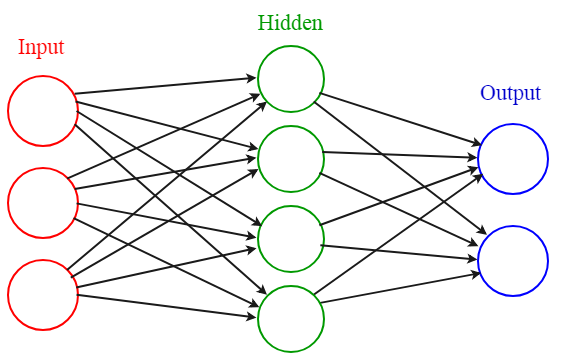
\includegraphics[height=0.35\linewidth]{./figures/feedforward}
	\caption{A neural network, where the circles represent the artificial neurons as nodes}
	\label{fig:feedforward}
\end{figure}

The artificial neural network itself is not an algorithm, but rather a framework for many different machine learning algorithms that can process complex data inputs. These learning algorithms learn from the experiences that are obtained from processing many examples. Each process yields an output, which, depending on the other outputs can determine which characteristics of the input are needed to construct the correct output. If there are a sufficient number of processed examples, the neural network can generate potential inputs and see if they produce the correct outputs. As the quantity of training data increases, so does the learning time and complexity of the neural network. However, training data also potentionally increases the estimation accuracy.



\subsection{ANN Inversion}

There is a subfield of machine learning that have not received much attention since the rise of deep learning. This subfield is the inversion problem \cite{KINDERMANN1990277}. \smallskip

\label{para:inversion}Neural network inversion procedures seek to find one or more input values that produce a desired output response for a fixed set of synaptic weights. \medskip

There are many methods which can perform neural network inversion. These can be placed into three broad classes. Exhaustive search should be considered when the dimensionality of the input and allowable range of each input variable is low. Single element inversion methods are used to find one inversion point per process. Multi-element inversion procedures are able to find numerous inversion points simultaneously. \medskip

Even if the inversion problem is not the most popular area in connection with neural networks, it has wide application areas. For example, a single element inversion task is the problem of sonar performance under various environmental conditions \cite{article}. 



\section{Python}

Python \cite{van2011introduction}\cite{vanderplas2016python} is an interpreted, object-oriented, high-level programming language with dynamic semantics, used for general-purpose programming. It was created by Guido van Rossum and released in 1991. \medskip

Python has became a preferred programming language over the last couple decades for scientific computing tasks, including the analysis and processing of large datasets. It is easy to learn, has efficient high-level data structures and a simple but effective approach to object-oriented programming.

\begin{figure}[h]
	\centering
	\caption{Python and its library Scikit-Learn are appropriate platforms to make artificial neural networks}
	
\includegraphics[height=0.25\linewidth]{./figures/python_scikit}
	\label{fig:python_scikit}
\end{figure}

In the artificial intelligence community, Python is one of the most used language. Researchers from numerous fields of artificial intelligence  develop in Python, with the assistance of the built-in libraries and other sources found on the internet. The usefulness of Python for data science comes primarily from the large and active third-party packages: 
\begin{verse}
	- \textbf{SciPy} for containing a wide array of numerical tools such as numerical integration and interpolation;
	
	- \textbf{Scikit-Learn} for providing a uniform toolkit for applying common machine learning algorithms to data;
	
	- \textbf{NumPy} for providing efficient storage and computing multi-dimensional data arrays;
	
	-  \textbf{Pandas} for providing a DataFrame object along with a powerful set of methods to manipulate, filter, group, and transform data; 
	
	- \textbf{Matplotlib} for providing a useful interface for creating publication-quality plots and figures;
\end{verse} 
and many more tools that aimed scientific computing and other machine learning fields.\\ 
Besides the prebuilt libraries, choosing Python for artificial intelligence programming can be faster with the specific indenting style and the dynamic typing system. Python is platform independent, its interpreter and extensive standard library are available in source or binary form for free.